\documentclass[11pt]{article}
\usepackage[textwidth=18.0cm, textheight=23.0cm, top=2.0cm]{geometry}
\usepackage{pst-all}
\usepackage{amssymb}
\usepackage{tikz}
\usepackage{underscore}\begin{document}
\pagestyle{empty}


ClassName: \underline{\textbf{Class_07.2bp-21}}
\par
BinSize: \underline{\textbf{100 × 100}}
\par
ReduceSize: \underline{\textbf{100 × 100}}
\par
TypeNum: \underline{\textbf{59}}
\par
Num: \underline{\textbf{60}}
\par
OutS: \underline{\textbf{140000}}
\par
InS: \underline{\textbf{123761}}
\par
Rate: \underline{\textbf{0.884}}
\par
UB: \underline{\textbf{14}}
\par
LB0: \underline{\textbf{14}}
\par
LB: \underline{\textbf{14}}
\par
LBWithCut: \underline{\textbf{14}}
\par
NodeCut: \underline{\textbf{0}}
\par
ExtendedNodeCnt: \underline{\textbf{1}}
\par
GenNodeCnt: \underline{\textbf{1}}
\par
PrimalNode: \underline{\textbf{0}}
\par
ColumnCount: \underline{\textbf{14}}
\par
TotalCutCount: \underline{\textbf{0}}
\par
RootCutCount: \underline{\textbf{0}}
\par
LPSolverCnt: \underline{\textbf{1}}
\par
PricingSolverCnt: \underline{\textbf{0}}
\par
BranchAndBoundNum: \underline{\textbf{1}}
\par
isOpt: \underline{\textbf{true}}
\par
TimeOnInitSolution: \underline{\textbf{600.000 s}}
\par
TimeOnPrimal: \underline{\textbf{0.000 s}}
\par
TimeOnPricing: \underline{\textbf{0.000 s}}
\par
TimeOnRmp: \underline{\textbf{0.079 s}}
\par
TotalTime: \underline{\textbf{600.360 s}}
\par
\newpage


\begin{tikzpicture}[shorten >=1pt,scale=1.0,every node/.style={scale=1.0},->]
\tikzstyle{vertex}=[circle,fill=black!25,minimum size=14pt,inner sep=0pt]
\filldraw[fill=gray!40!white, draw=black] (0,0) rectangle (15.0,15.0);
\foreach \name/\x/\y/\w/\h in {48x100/7.8/0.0/7.199999999999999/15.0,19x100/4.95/0.0/2.85/15.0,14x100/2.85/0.0/2.1/15.0,13x98/0.8999999999999999/0.0/1.95/14.7,6x96/0.0/0.0/0.8999999999999999/14.399999999999999}
\filldraw[fill=white!40!white, draw=black] (\x,\y) rectangle node[draw] (\name) {\name} ++(\w,\h);
\end{tikzpicture}


w =48 , h =100 , x =52 , y =0 , v =4800
\par
w =19 , h =100 , x =33 , y =0 , v =1900
\par
w =14 , h =100 , x =19 , y =0 , v =1400
\par
w =13 , h =98 , x =6 , y =0 , v =1274
\par
w =6 , h =96 , x =0 , y =0 , v =576
\par
\newpage


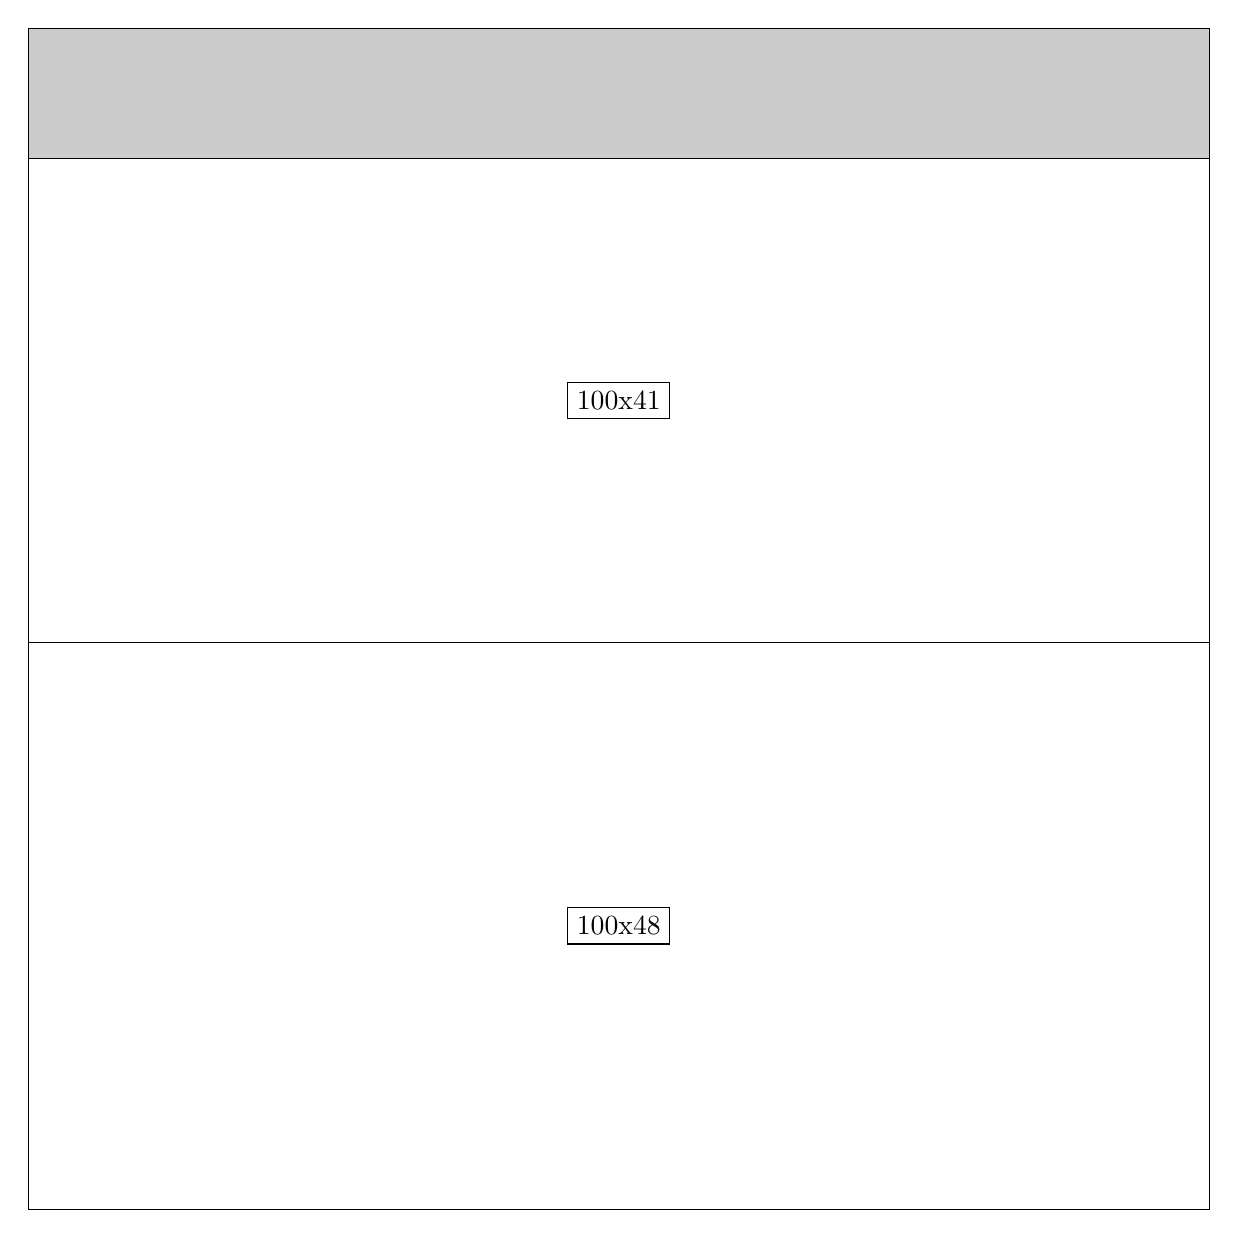
\begin{tikzpicture}[shorten >=1pt,scale=1.0,every node/.style={scale=1.0},->]
\tikzstyle{vertex}=[circle,fill=black!25,minimum size=14pt,inner sep=0pt]
\filldraw[fill=gray!40!white, draw=black] (0,0) rectangle (15.0,15.0);
\foreach \name/\x/\y/\w/\h in {100x48/0.0/0.0/15.0/7.199999999999999,100x41/0.0/7.199999999999999/15.0/6.1499999999999995}
\filldraw[fill=white!40!white, draw=black] (\x,\y) rectangle node[draw] (\name) {\name} ++(\w,\h);
\end{tikzpicture}


w =100 , h =48 , x =0 , y =0 , v =4800
\par
w =100 , h =41 , x =0 , y =48 , v =4100
\par
\newpage


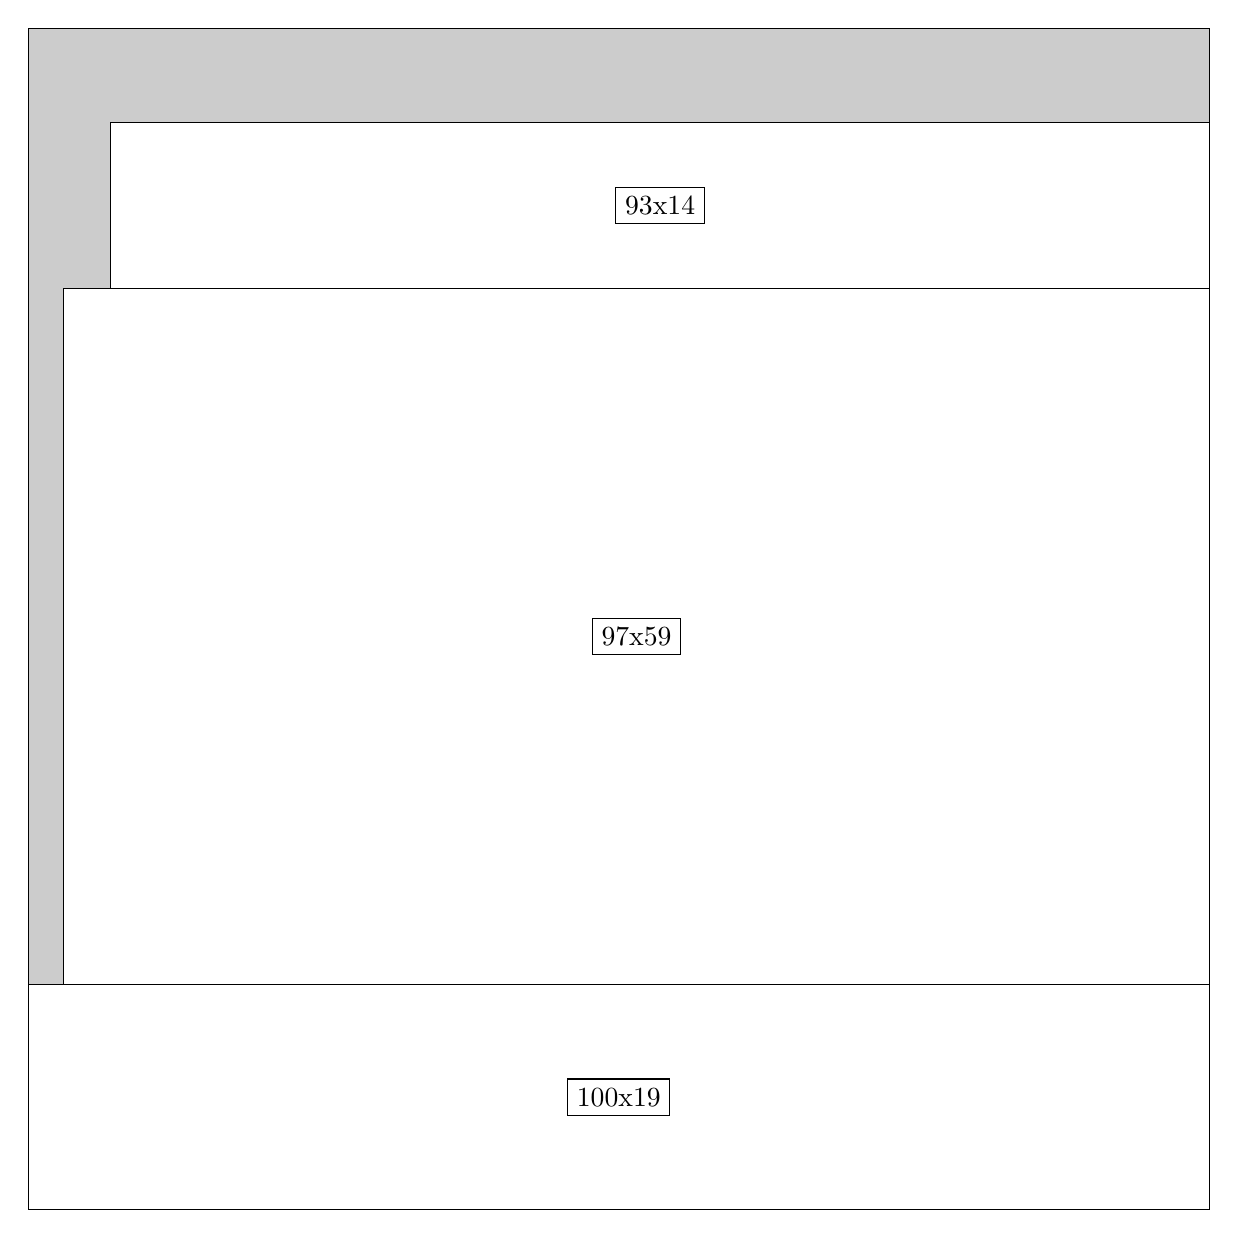
\begin{tikzpicture}[shorten >=1pt,scale=1.0,every node/.style={scale=1.0},->]
\tikzstyle{vertex}=[circle,fill=black!25,minimum size=14pt,inner sep=0pt]
\filldraw[fill=gray!40!white, draw=black] (0,0) rectangle (15.0,15.0);
\foreach \name/\x/\y/\w/\h in {100x19/0.0/0.0/15.0/2.85,97x59/0.44999999999999996/2.85/14.549999999999999/8.85,93x14/1.05/11.7/13.95/2.1}
\filldraw[fill=white!40!white, draw=black] (\x,\y) rectangle node[draw] (\name) {\name} ++(\w,\h);
\end{tikzpicture}


w =100 , h =19 , x =0 , y =0 , v =1900
\par
w =97 , h =59 , x =3 , y =19 , v =5723
\par
w =93 , h =14 , x =7 , y =78 , v =1302
\par
\newpage


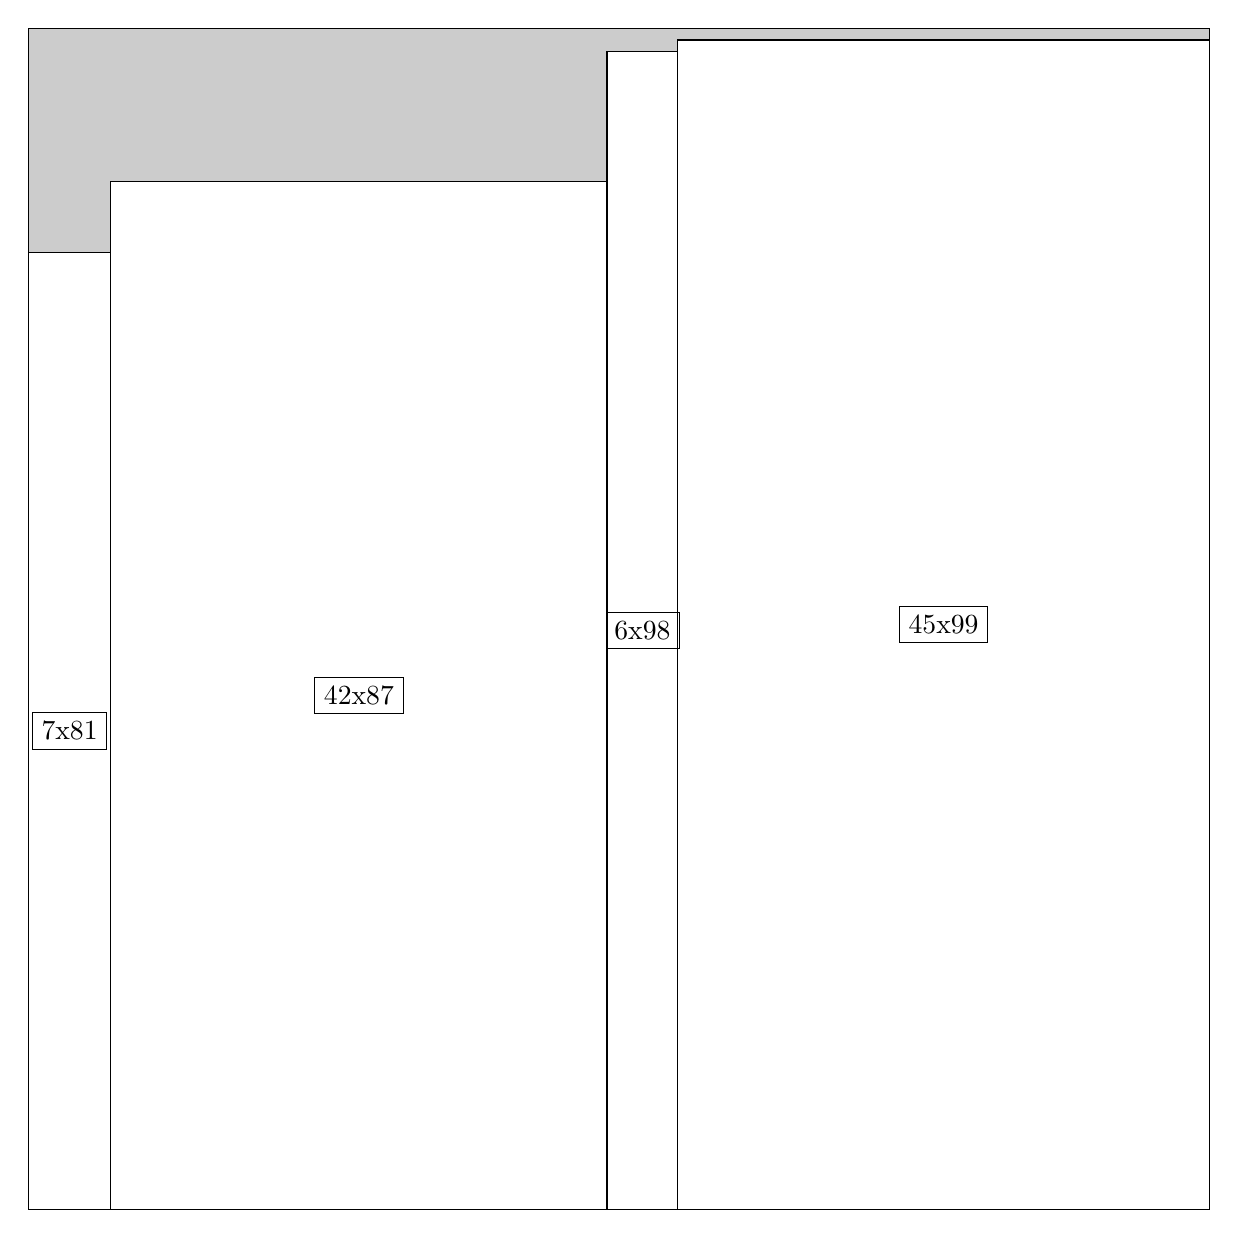
\begin{tikzpicture}[shorten >=1pt,scale=1.0,every node/.style={scale=1.0},->]
\tikzstyle{vertex}=[circle,fill=black!25,minimum size=14pt,inner sep=0pt]
\filldraw[fill=gray!40!white, draw=black] (0,0) rectangle (15.0,15.0);
\foreach \name/\x/\y/\w/\h in {45x99/8.25/0.0/6.75/14.85,6x98/7.35/0.0/0.8999999999999999/14.7,42x87/1.05/0.0/6.3/13.049999999999999,7x81/0.0/0.0/1.05/12.15}
\filldraw[fill=white!40!white, draw=black] (\x,\y) rectangle node[draw] (\name) {\name} ++(\w,\h);
\end{tikzpicture}


w =45 , h =99 , x =55 , y =0 , v =4455
\par
w =6 , h =98 , x =49 , y =0 , v =588
\par
w =42 , h =87 , x =7 , y =0 , v =3654
\par
w =7 , h =81 , x =0 , y =0 , v =567
\par
\newpage


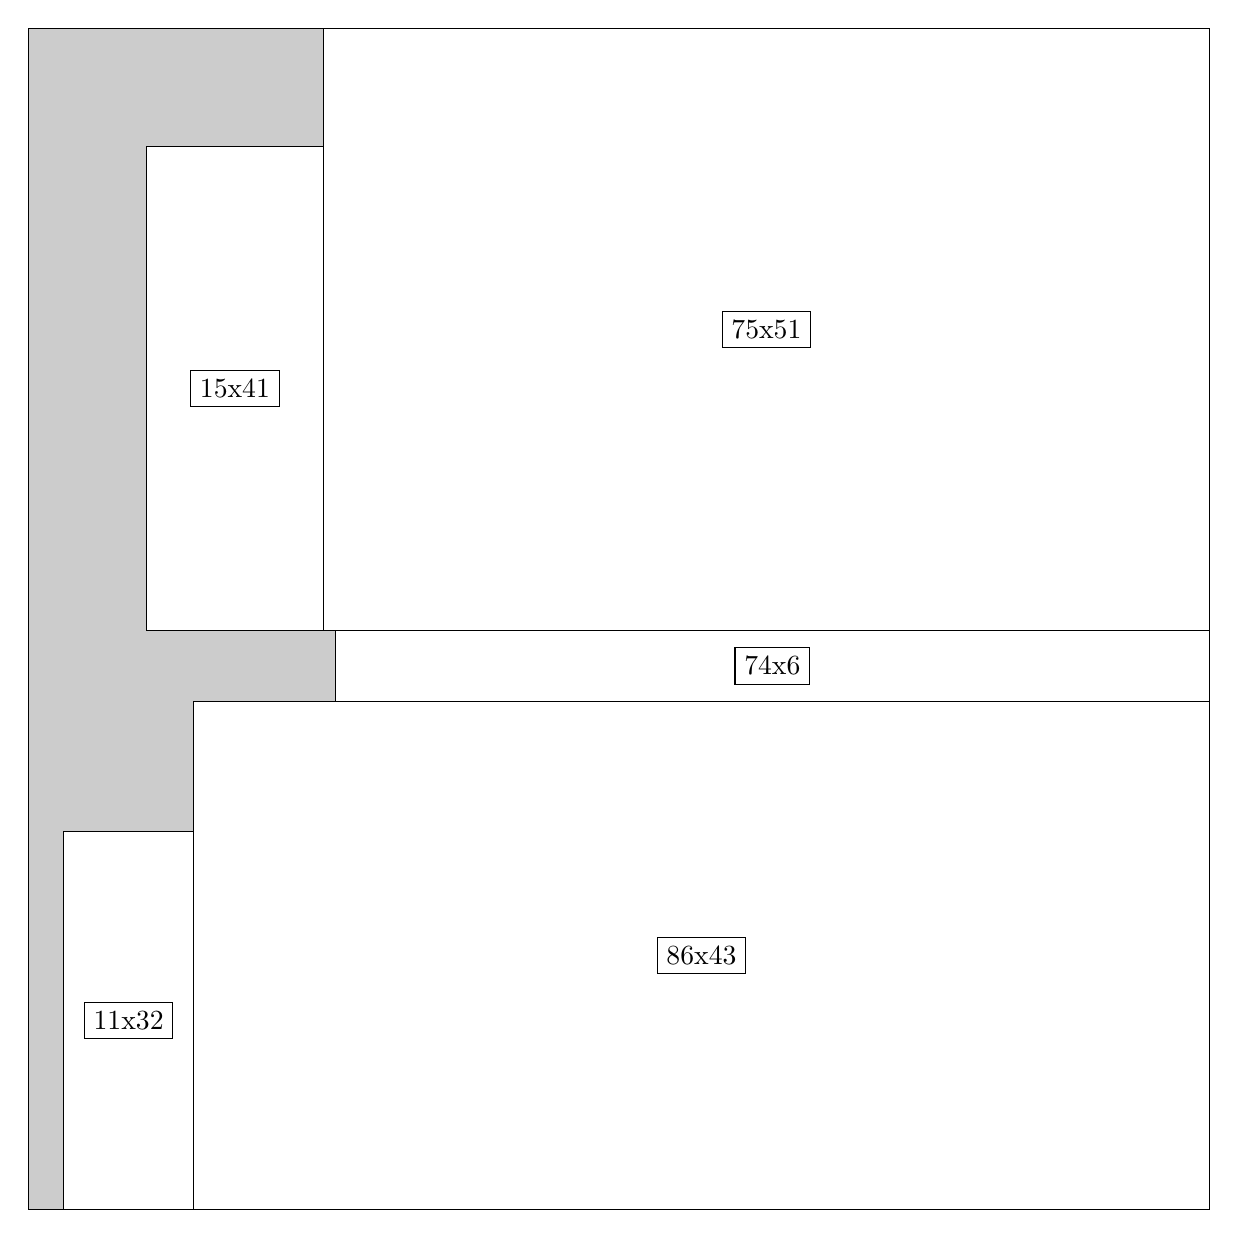
\begin{tikzpicture}[shorten >=1pt,scale=1.0,every node/.style={scale=1.0},->]
\tikzstyle{vertex}=[circle,fill=black!25,minimum size=14pt,inner sep=0pt]
\filldraw[fill=gray!40!white, draw=black] (0,0) rectangle (15.0,15.0);
\foreach \name/\x/\y/\w/\h in {86x43/2.1/0.0/12.9/6.45,74x6/3.9/6.45/11.1/0.8999999999999999,11x32/0.44999999999999996/0.0/1.65/4.8,75x51/3.75/7.35/11.25/7.6499999999999995,15x41/1.5/7.35/2.25/6.1499999999999995}
\filldraw[fill=white!40!white, draw=black] (\x,\y) rectangle node[draw] (\name) {\name} ++(\w,\h);
\end{tikzpicture}


w =86 , h =43 , x =14 , y =0 , v =3698
\par
w =74 , h =6 , x =26 , y =43 , v =444
\par
w =11 , h =32 , x =3 , y =0 , v =352
\par
w =75 , h =51 , x =25 , y =49 , v =3825
\par
w =15 , h =41 , x =10 , y =49 , v =615
\par
\newpage


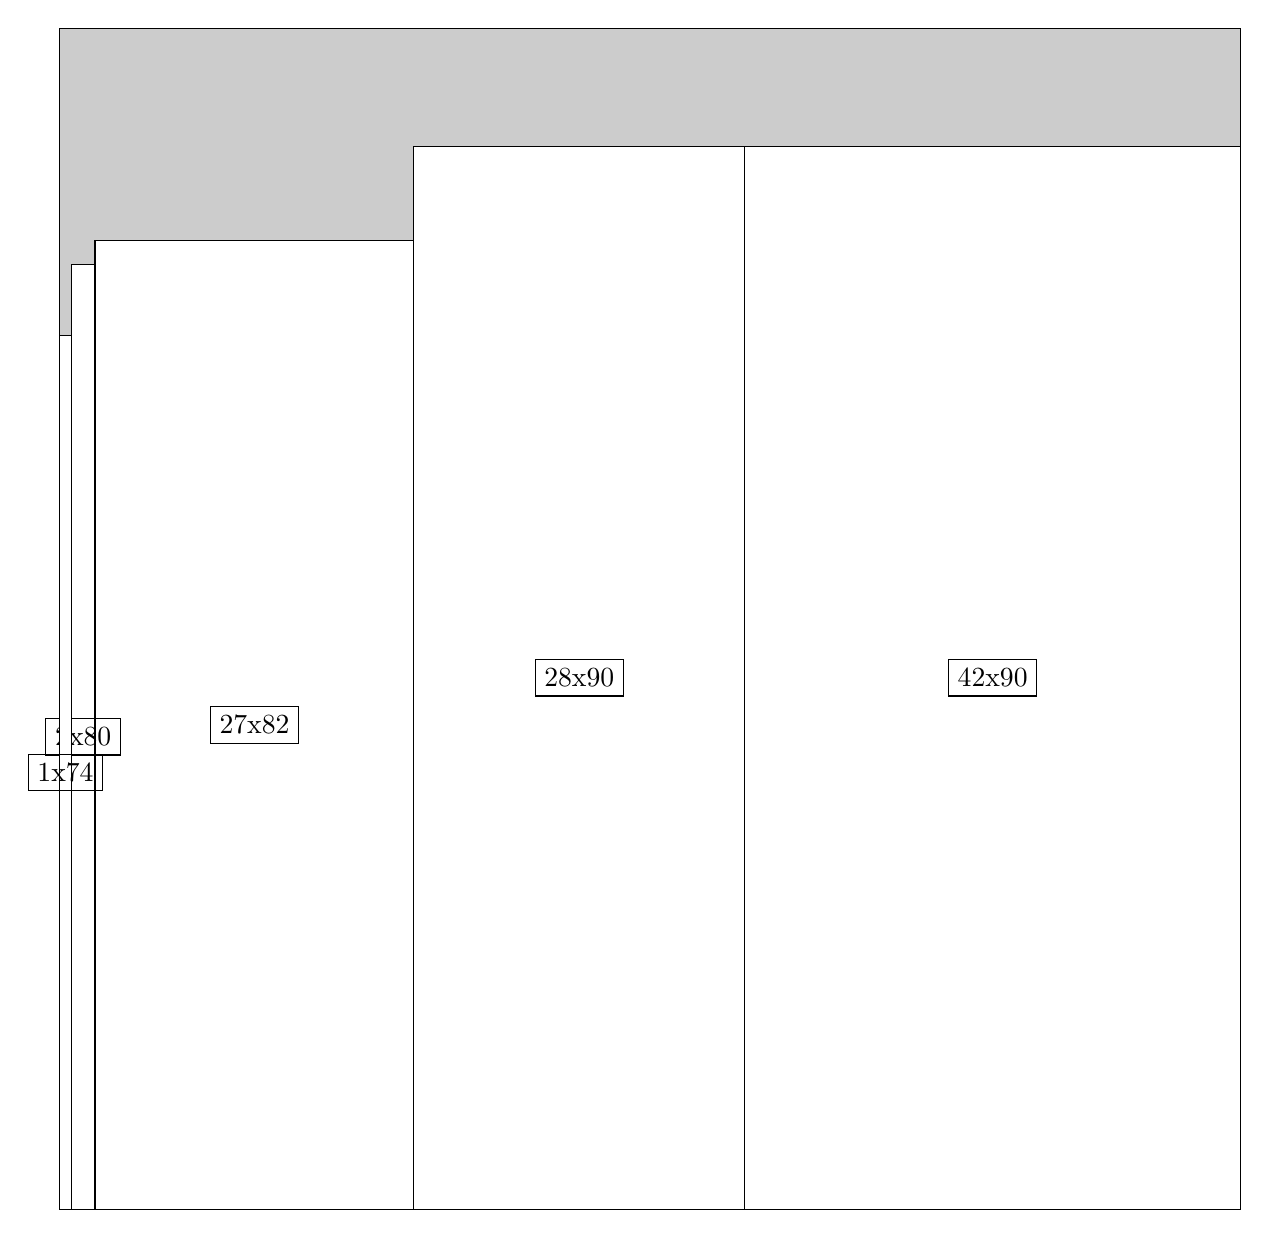
\begin{tikzpicture}[shorten >=1pt,scale=1.0,every node/.style={scale=1.0},->]
\tikzstyle{vertex}=[circle,fill=black!25,minimum size=14pt,inner sep=0pt]
\filldraw[fill=gray!40!white, draw=black] (0,0) rectangle (15.0,15.0);
\foreach \name/\x/\y/\w/\h in {42x90/8.7/0.0/6.3/13.5,28x90/4.5/0.0/4.2/13.5,27x82/0.44999999999999996/0.0/4.05/12.299999999999999,2x80/0.15/0.0/0.3/12.0,1x74/0.0/0.0/0.15/11.1}
\filldraw[fill=white!40!white, draw=black] (\x,\y) rectangle node[draw] (\name) {\name} ++(\w,\h);
\end{tikzpicture}


w =42 , h =90 , x =58 , y =0 , v =3780
\par
w =28 , h =90 , x =30 , y =0 , v =2520
\par
w =27 , h =82 , x =3 , y =0 , v =2214
\par
w =2 , h =80 , x =1 , y =0 , v =160
\par
w =1 , h =74 , x =0 , y =0 , v =74
\par
\newpage


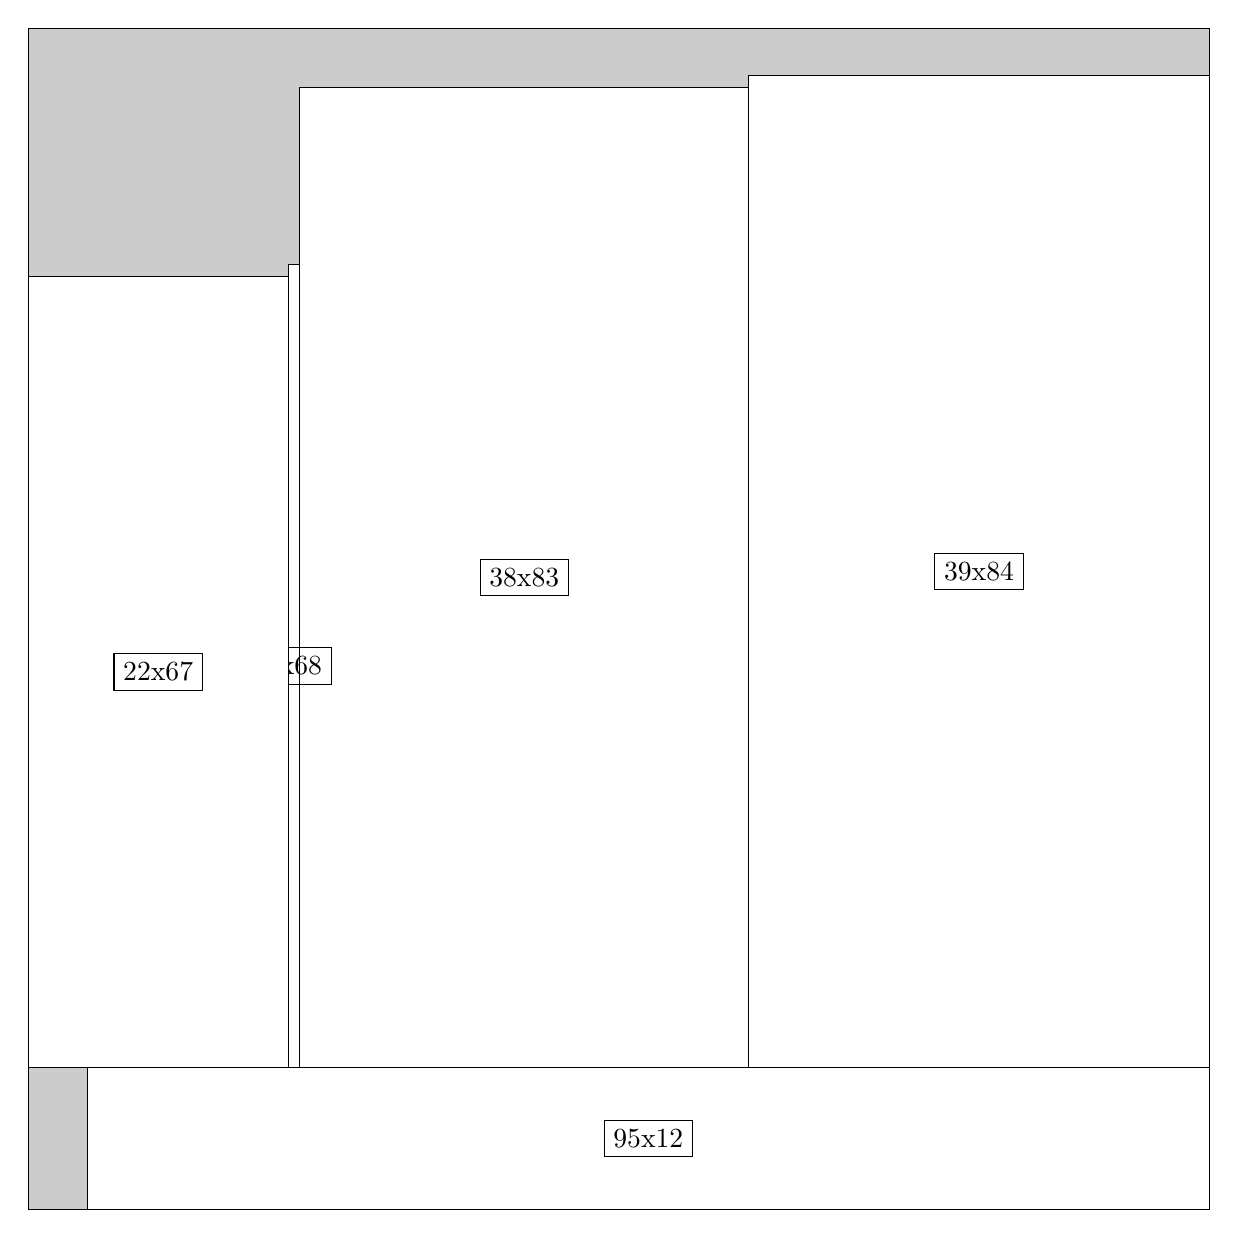
\begin{tikzpicture}[shorten >=1pt,scale=1.0,every node/.style={scale=1.0},->]
\tikzstyle{vertex}=[circle,fill=black!25,minimum size=14pt,inner sep=0pt]
\filldraw[fill=gray!40!white, draw=black] (0,0) rectangle (15.0,15.0);
\foreach \name/\x/\y/\w/\h in {95x12/0.75/0.0/14.25/1.7999999999999998,39x84/9.15/1.7999999999999998/5.85/12.6,38x83/3.4499999999999997/1.7999999999999998/5.7/12.45,1x68/3.3/1.7999999999999998/0.15/10.2,22x67/0.0/1.7999999999999998/3.3/10.049999999999999}
\filldraw[fill=white!40!white, draw=black] (\x,\y) rectangle node[draw] (\name) {\name} ++(\w,\h);
\end{tikzpicture}


w =95 , h =12 , x =5 , y =0 , v =1140
\par
w =39 , h =84 , x =61 , y =12 , v =3276
\par
w =38 , h =83 , x =23 , y =12 , v =3154
\par
w =1 , h =68 , x =22 , y =12 , v =68
\par
w =22 , h =67 , x =0 , y =12 , v =1474
\par
\newpage


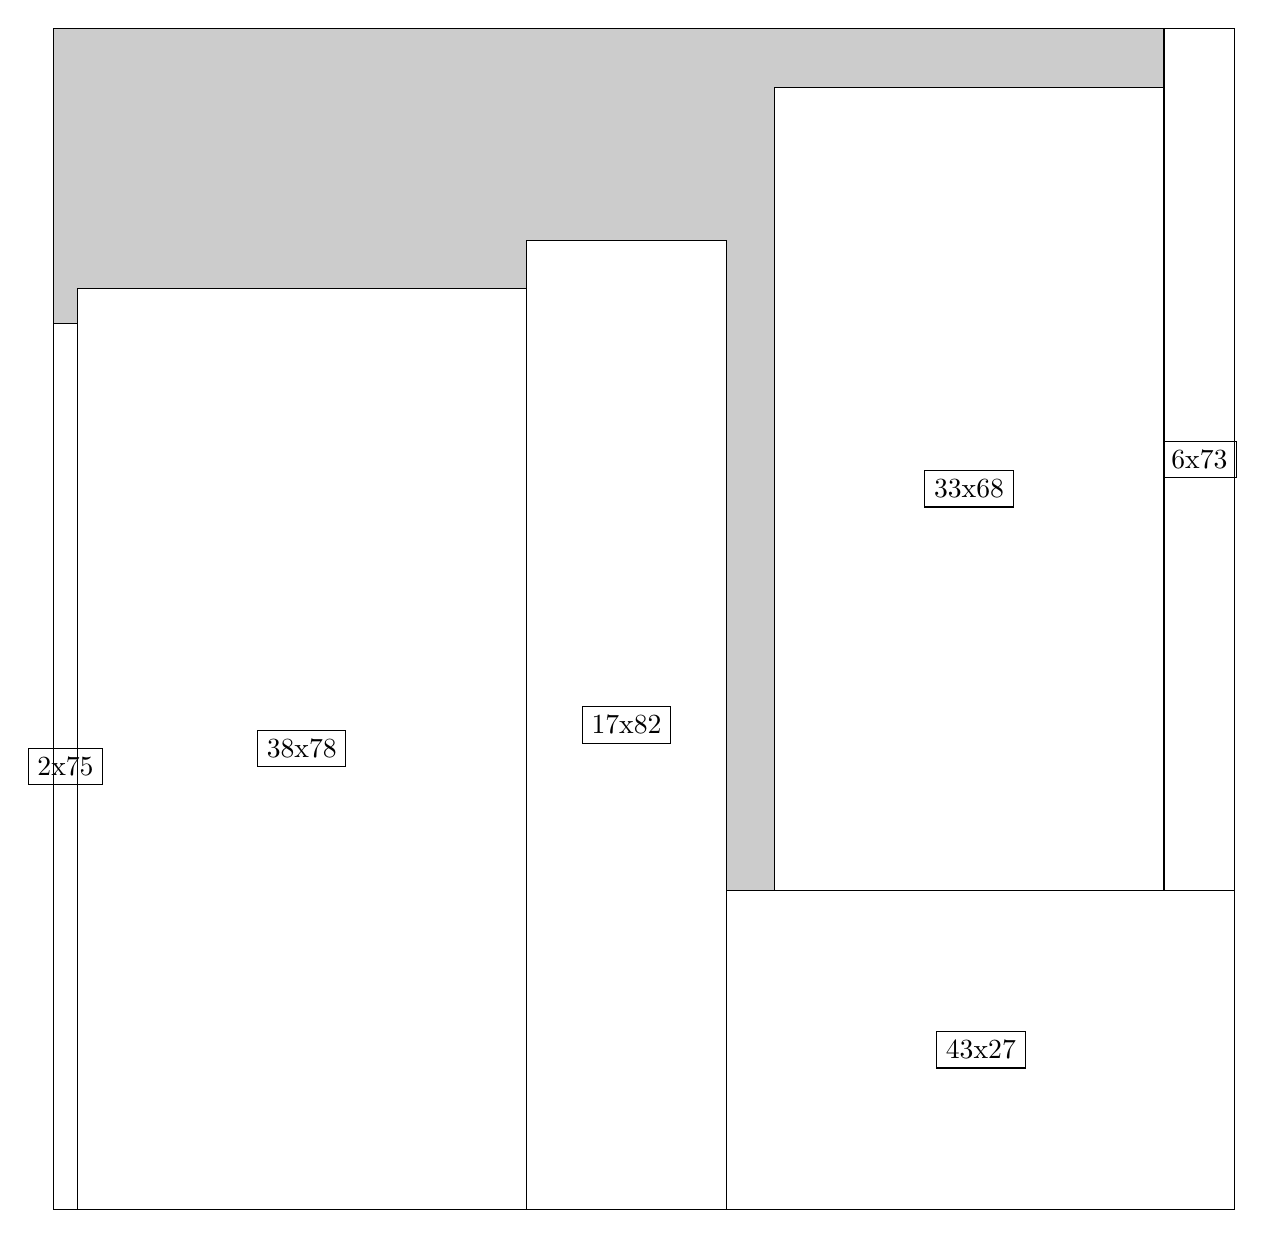
\begin{tikzpicture}[shorten >=1pt,scale=1.0,every node/.style={scale=1.0},->]
\tikzstyle{vertex}=[circle,fill=black!25,minimum size=14pt,inner sep=0pt]
\filldraw[fill=gray!40!white, draw=black] (0,0) rectangle (15.0,15.0);
\foreach \name/\x/\y/\w/\h in {43x27/8.549999999999999/0.0/6.45/4.05,6x73/14.1/4.05/0.8999999999999999/10.95,33x68/9.15/4.05/4.95/10.2,17x82/6.0/0.0/2.55/12.299999999999999,38x78/0.3/0.0/5.7/11.7,2x75/0.0/0.0/0.3/11.25}
\filldraw[fill=white!40!white, draw=black] (\x,\y) rectangle node[draw] (\name) {\name} ++(\w,\h);
\end{tikzpicture}


w =43 , h =27 , x =57 , y =0 , v =1161
\par
w =6 , h =73 , x =94 , y =27 , v =438
\par
w =33 , h =68 , x =61 , y =27 , v =2244
\par
w =17 , h =82 , x =40 , y =0 , v =1394
\par
w =38 , h =78 , x =2 , y =0 , v =2964
\par
w =2 , h =75 , x =0 , y =0 , v =150
\par
\newpage


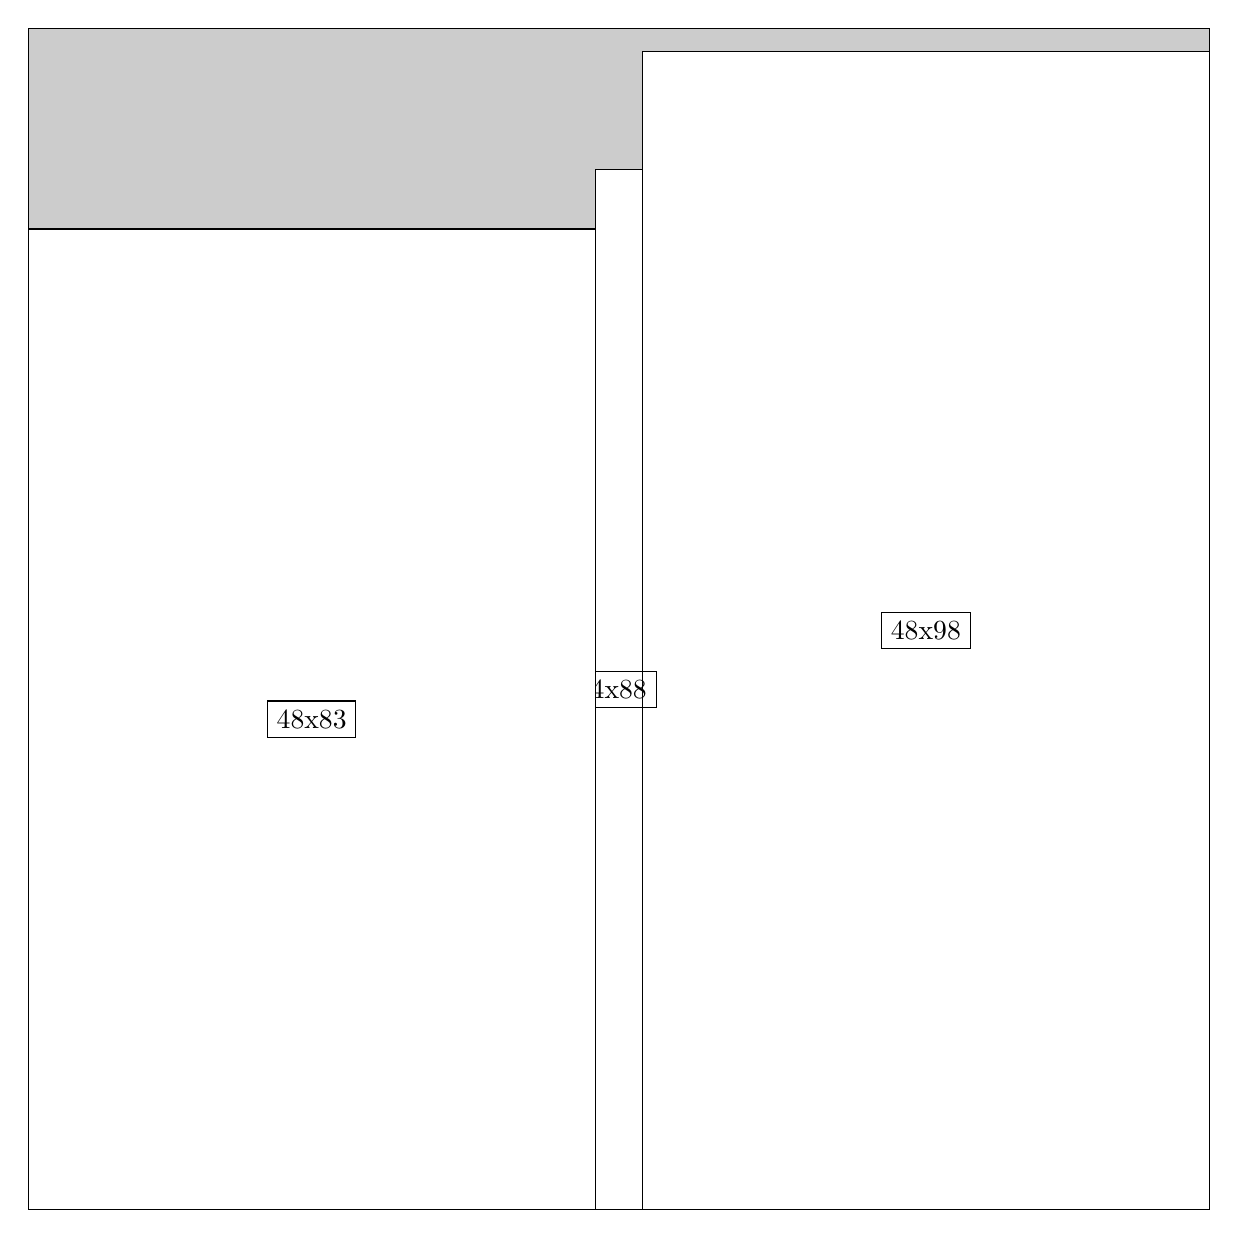
\begin{tikzpicture}[shorten >=1pt,scale=1.0,every node/.style={scale=1.0},->]
\tikzstyle{vertex}=[circle,fill=black!25,minimum size=14pt,inner sep=0pt]
\filldraw[fill=gray!40!white, draw=black] (0,0) rectangle (15.0,15.0);
\foreach \name/\x/\y/\w/\h in {48x98/7.8/0.0/7.199999999999999/14.7,4x88/7.199999999999999/0.0/0.6/13.2,48x83/0.0/0.0/7.199999999999999/12.45}
\filldraw[fill=white!40!white, draw=black] (\x,\y) rectangle node[draw] (\name) {\name} ++(\w,\h);
\end{tikzpicture}


w =48 , h =98 , x =52 , y =0 , v =4704
\par
w =4 , h =88 , x =48 , y =0 , v =352
\par
w =48 , h =83 , x =0 , y =0 , v =3984
\par
\newpage


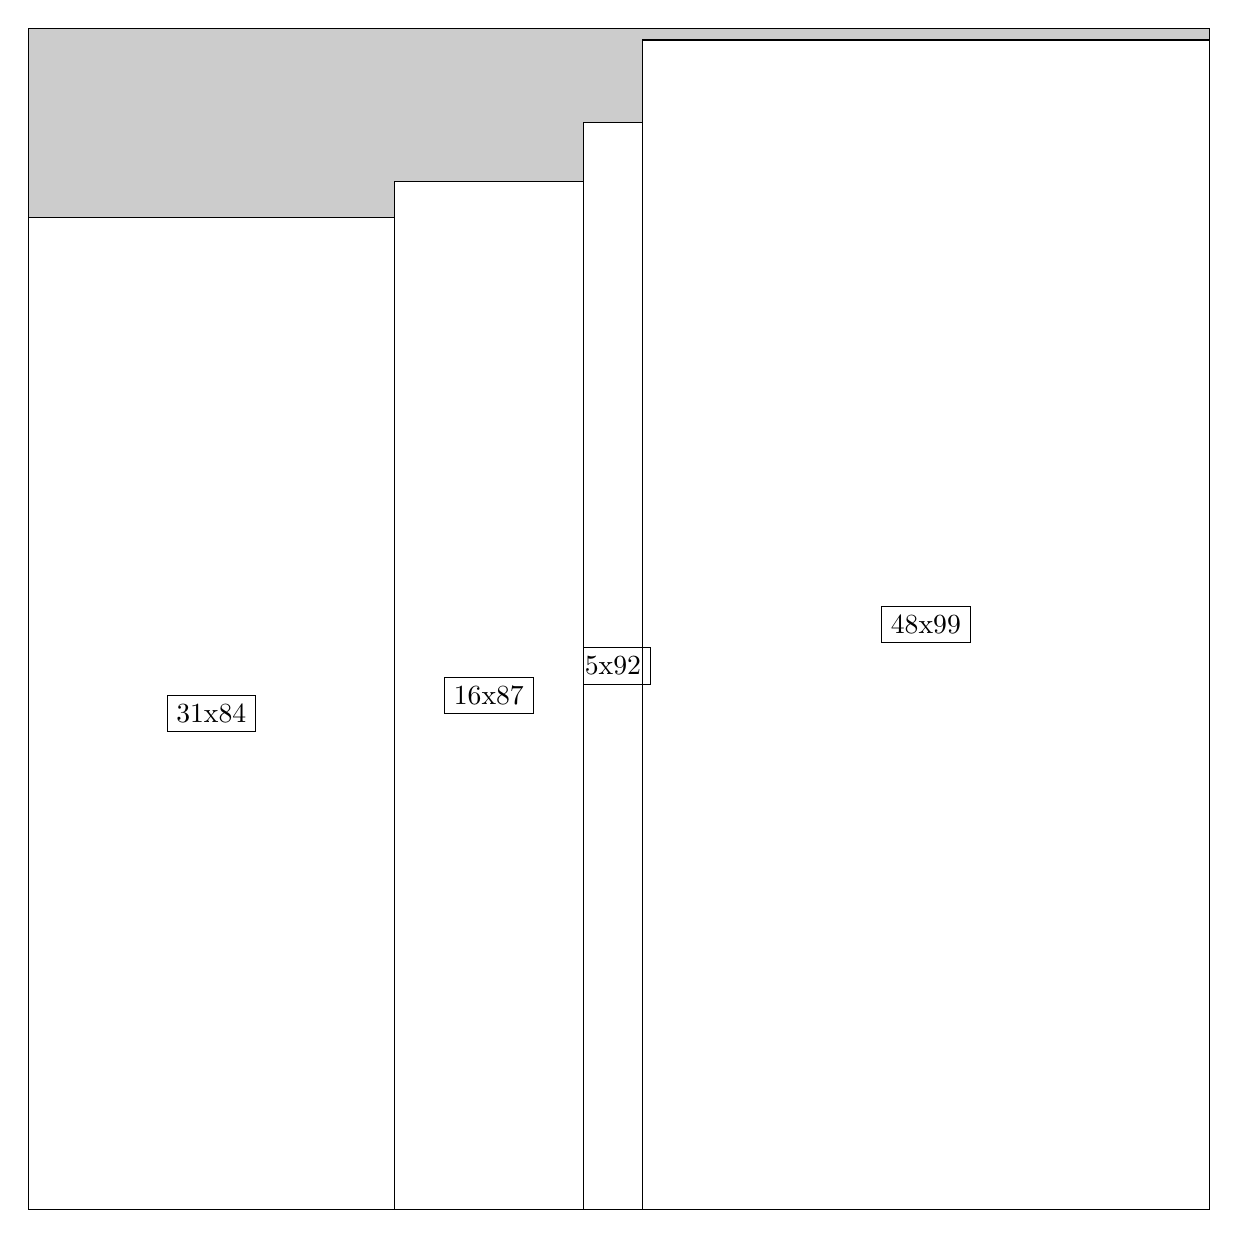
\begin{tikzpicture}[shorten >=1pt,scale=1.0,every node/.style={scale=1.0},->]
\tikzstyle{vertex}=[circle,fill=black!25,minimum size=14pt,inner sep=0pt]
\filldraw[fill=gray!40!white, draw=black] (0,0) rectangle (15.0,15.0);
\foreach \name/\x/\y/\w/\h in {48x99/7.8/0.0/7.199999999999999/14.85,5x92/7.05/0.0/0.75/13.799999999999999,16x87/4.6499999999999995/0.0/2.4/13.049999999999999,31x84/0.0/0.0/4.6499999999999995/12.6}
\filldraw[fill=white!40!white, draw=black] (\x,\y) rectangle node[draw] (\name) {\name} ++(\w,\h);
\end{tikzpicture}


w =48 , h =99 , x =52 , y =0 , v =4752
\par
w =5 , h =92 , x =47 , y =0 , v =460
\par
w =16 , h =87 , x =31 , y =0 , v =1392
\par
w =31 , h =84 , x =0 , y =0 , v =2604
\par
\newpage


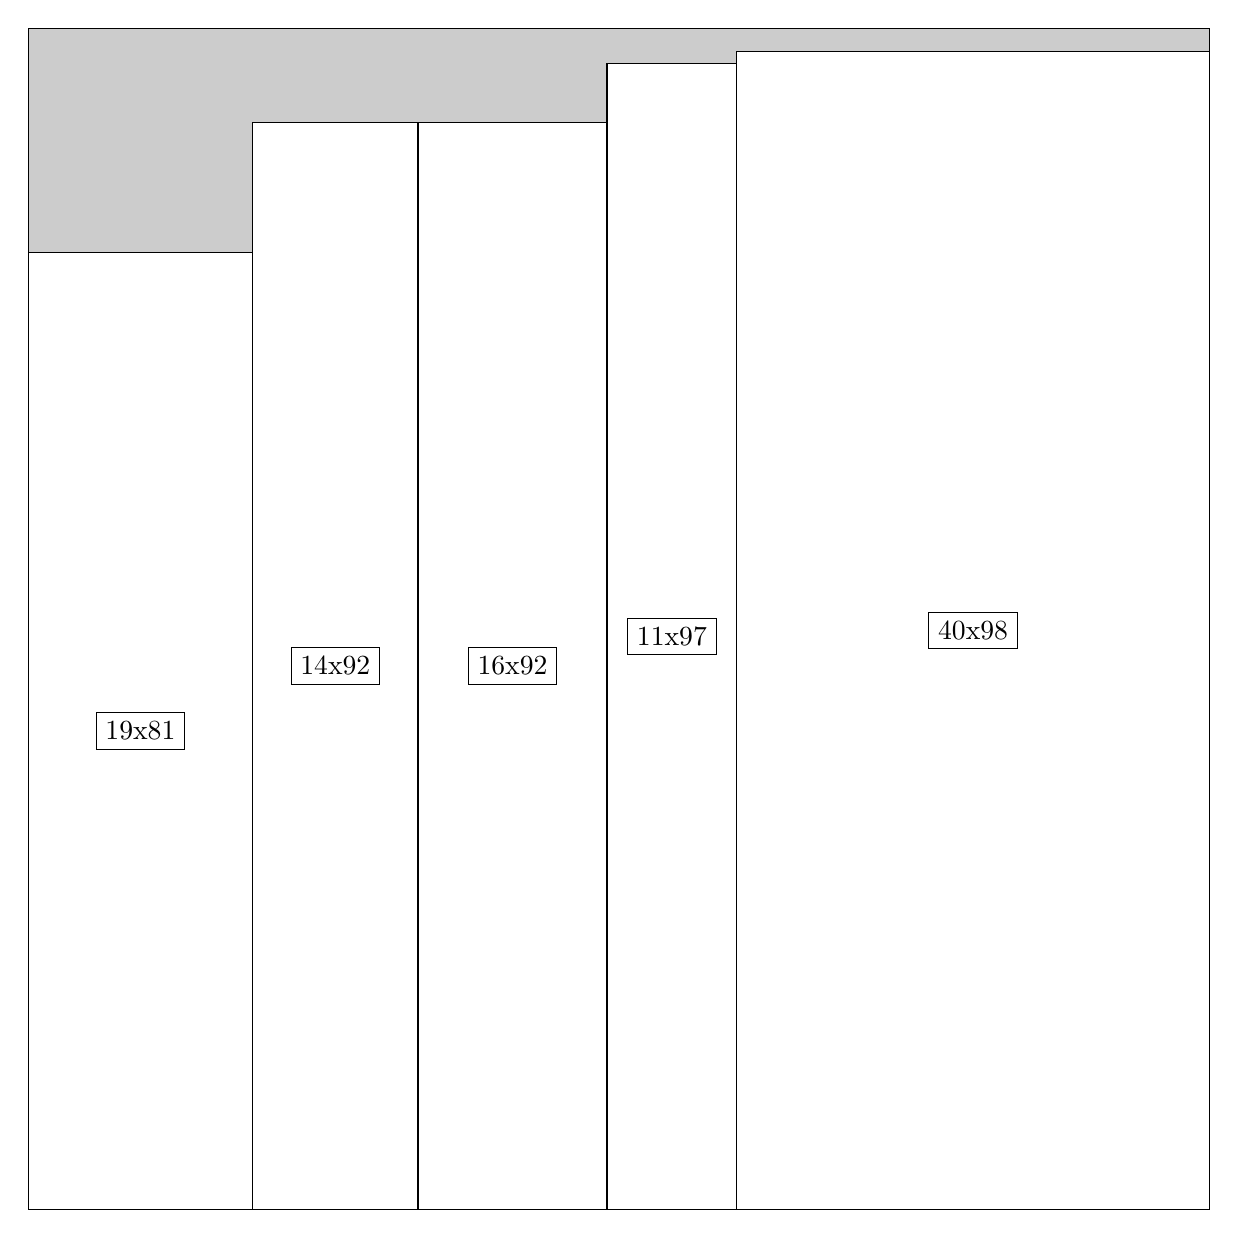
\begin{tikzpicture}[shorten >=1pt,scale=1.0,every node/.style={scale=1.0},->]
\tikzstyle{vertex}=[circle,fill=black!25,minimum size=14pt,inner sep=0pt]
\filldraw[fill=gray!40!white, draw=black] (0,0) rectangle (15.0,15.0);
\foreach \name/\x/\y/\w/\h in {40x98/9.0/0.0/6.0/14.7,11x97/7.35/0.0/1.65/14.549999999999999,16x92/4.95/0.0/2.4/13.799999999999999,14x92/2.85/0.0/2.1/13.799999999999999,19x81/0.0/0.0/2.85/12.15}
\filldraw[fill=white!40!white, draw=black] (\x,\y) rectangle node[draw] (\name) {\name} ++(\w,\h);
\end{tikzpicture}


w =40 , h =98 , x =60 , y =0 , v =3920
\par
w =11 , h =97 , x =49 , y =0 , v =1067
\par
w =16 , h =92 , x =33 , y =0 , v =1472
\par
w =14 , h =92 , x =19 , y =0 , v =1288
\par
w =19 , h =81 , x =0 , y =0 , v =1539
\par
\newpage


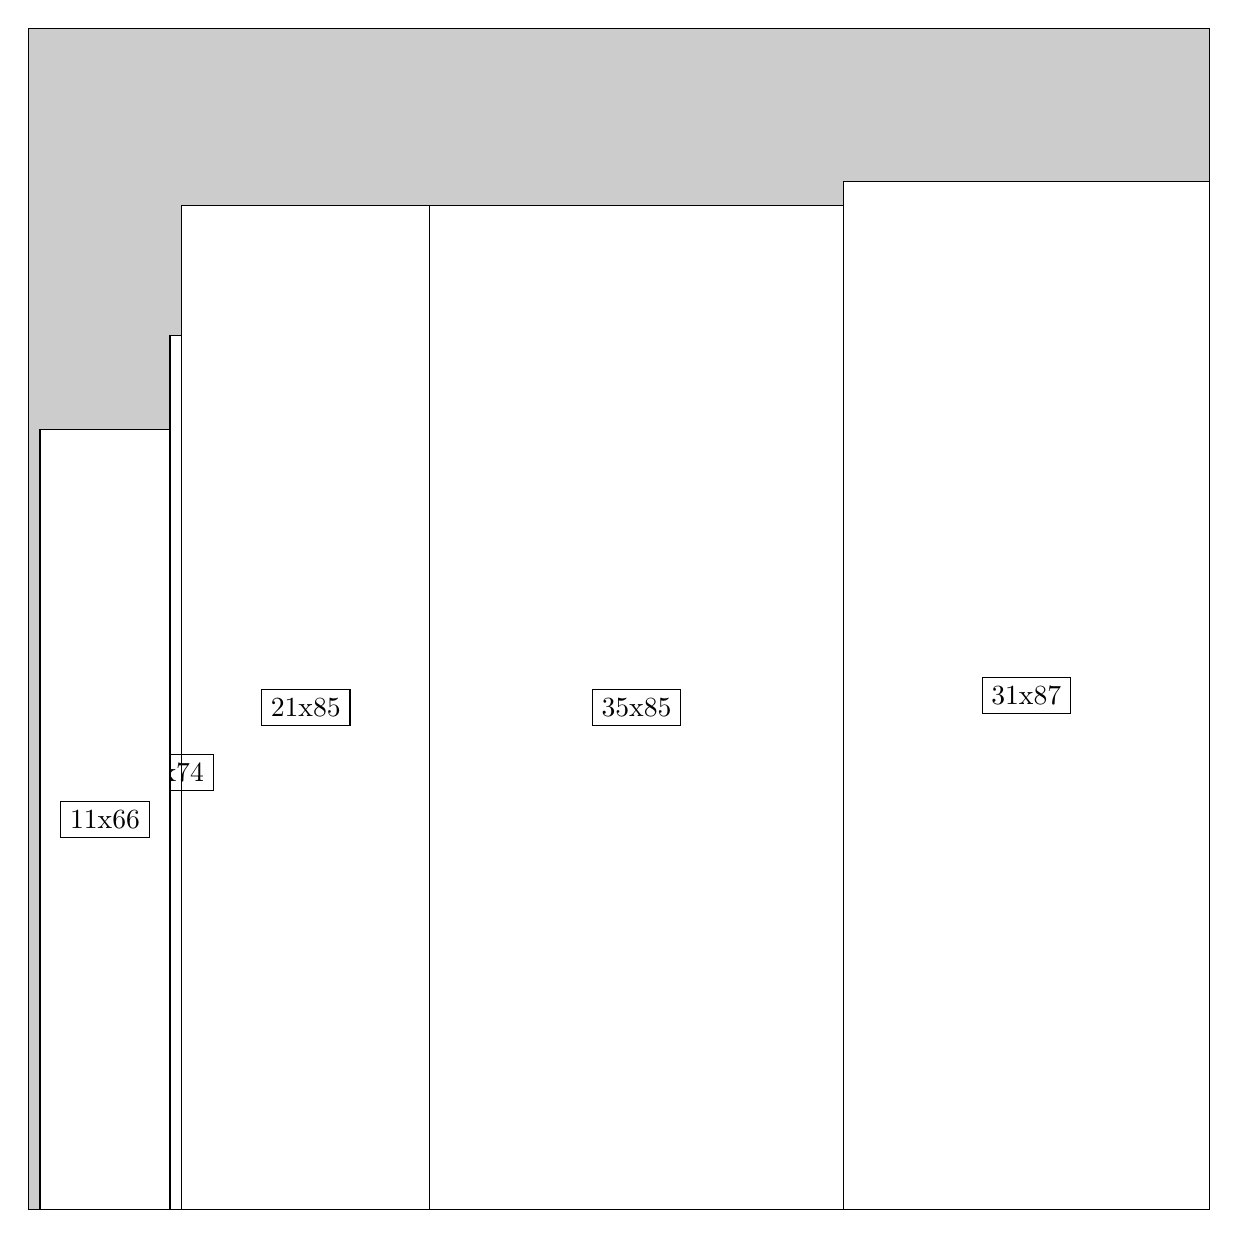
\begin{tikzpicture}[shorten >=1pt,scale=1.0,every node/.style={scale=1.0},->]
\tikzstyle{vertex}=[circle,fill=black!25,minimum size=14pt,inner sep=0pt]
\filldraw[fill=gray!40!white, draw=black] (0,0) rectangle (15.0,15.0);
\foreach \name/\x/\y/\w/\h in {31x87/10.35/0.0/4.6499999999999995/13.049999999999999,35x85/5.1/0.0/5.25/12.75,21x85/1.95/0.0/3.15/12.75,1x74/1.7999999999999998/0.0/0.15/11.1,11x66/0.15/0.0/1.65/9.9}
\filldraw[fill=white!40!white, draw=black] (\x,\y) rectangle node[draw] (\name) {\name} ++(\w,\h);
\end{tikzpicture}


w =31 , h =87 , x =69 , y =0 , v =2697
\par
w =35 , h =85 , x =34 , y =0 , v =2975
\par
w =21 , h =85 , x =13 , y =0 , v =1785
\par
w =1 , h =74 , x =12 , y =0 , v =74
\par
w =11 , h =66 , x =1 , y =0 , v =726
\par
\newpage


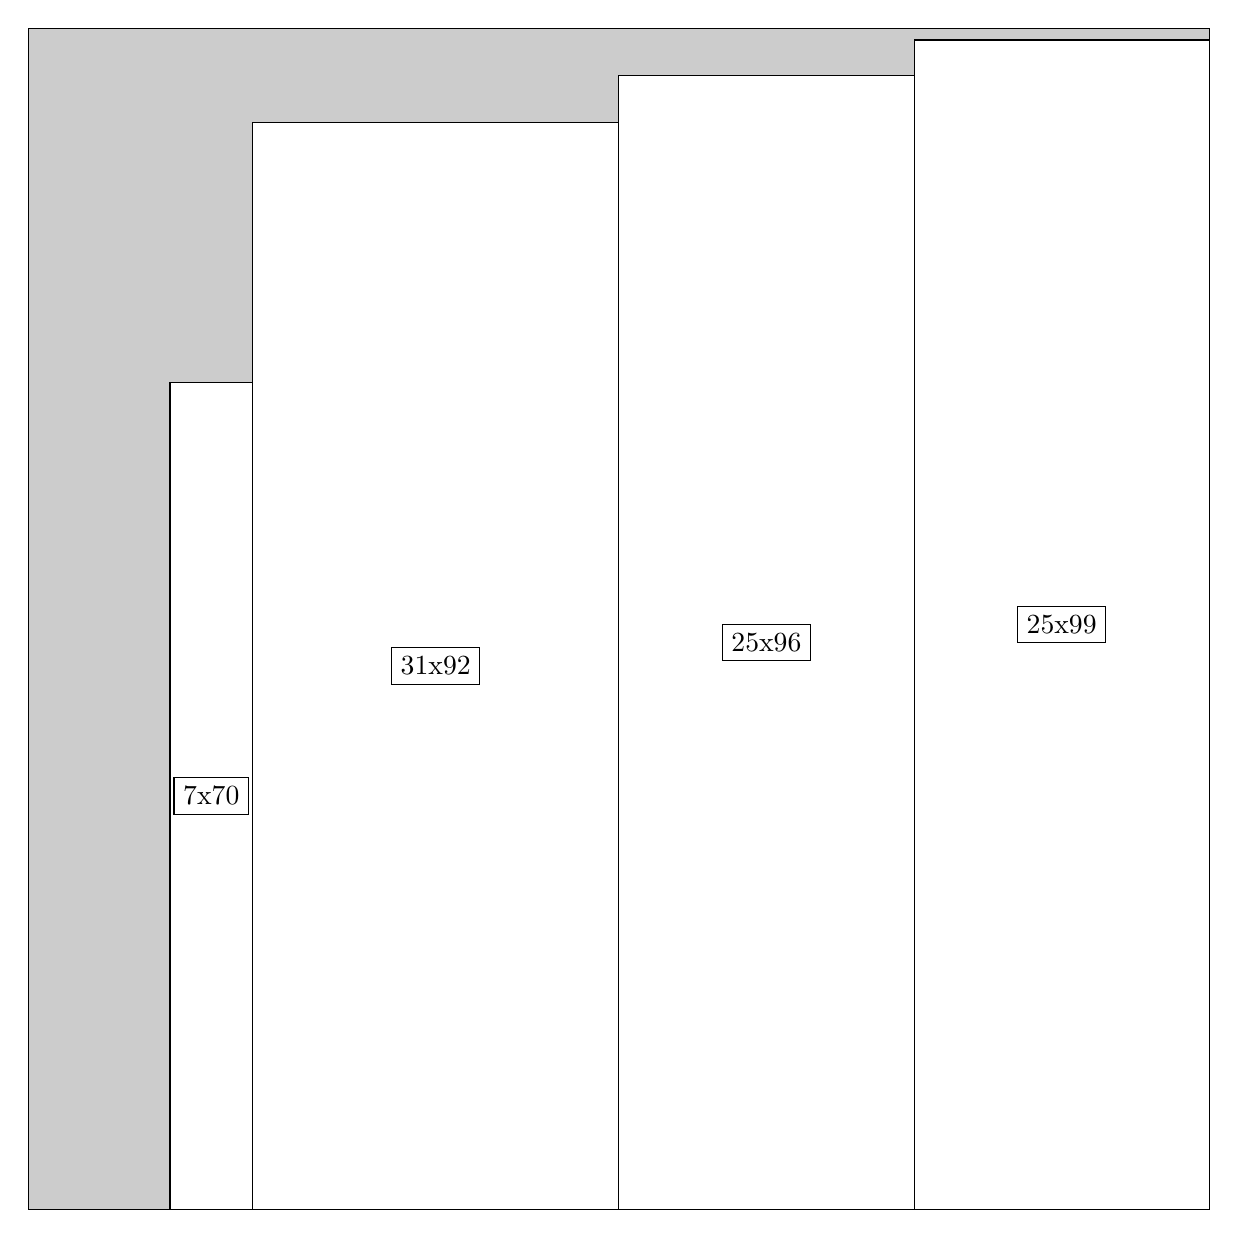
\begin{tikzpicture}[shorten >=1pt,scale=1.0,every node/.style={scale=1.0},->]
\tikzstyle{vertex}=[circle,fill=black!25,minimum size=14pt,inner sep=0pt]
\filldraw[fill=gray!40!white, draw=black] (0,0) rectangle (15.0,15.0);
\foreach \name/\x/\y/\w/\h in {25x99/11.25/0.0/3.75/14.85,25x96/7.5/0.0/3.75/14.399999999999999,31x92/2.85/0.0/4.6499999999999995/13.799999999999999,7x70/1.7999999999999998/0.0/1.05/10.5}
\filldraw[fill=white!40!white, draw=black] (\x,\y) rectangle node[draw] (\name) {\name} ++(\w,\h);
\end{tikzpicture}


w =25 , h =99 , x =75 , y =0 , v =2475
\par
w =25 , h =96 , x =50 , y =0 , v =2400
\par
w =31 , h =92 , x =19 , y =0 , v =2852
\par
w =7 , h =70 , x =12 , y =0 , v =490
\par
\newpage


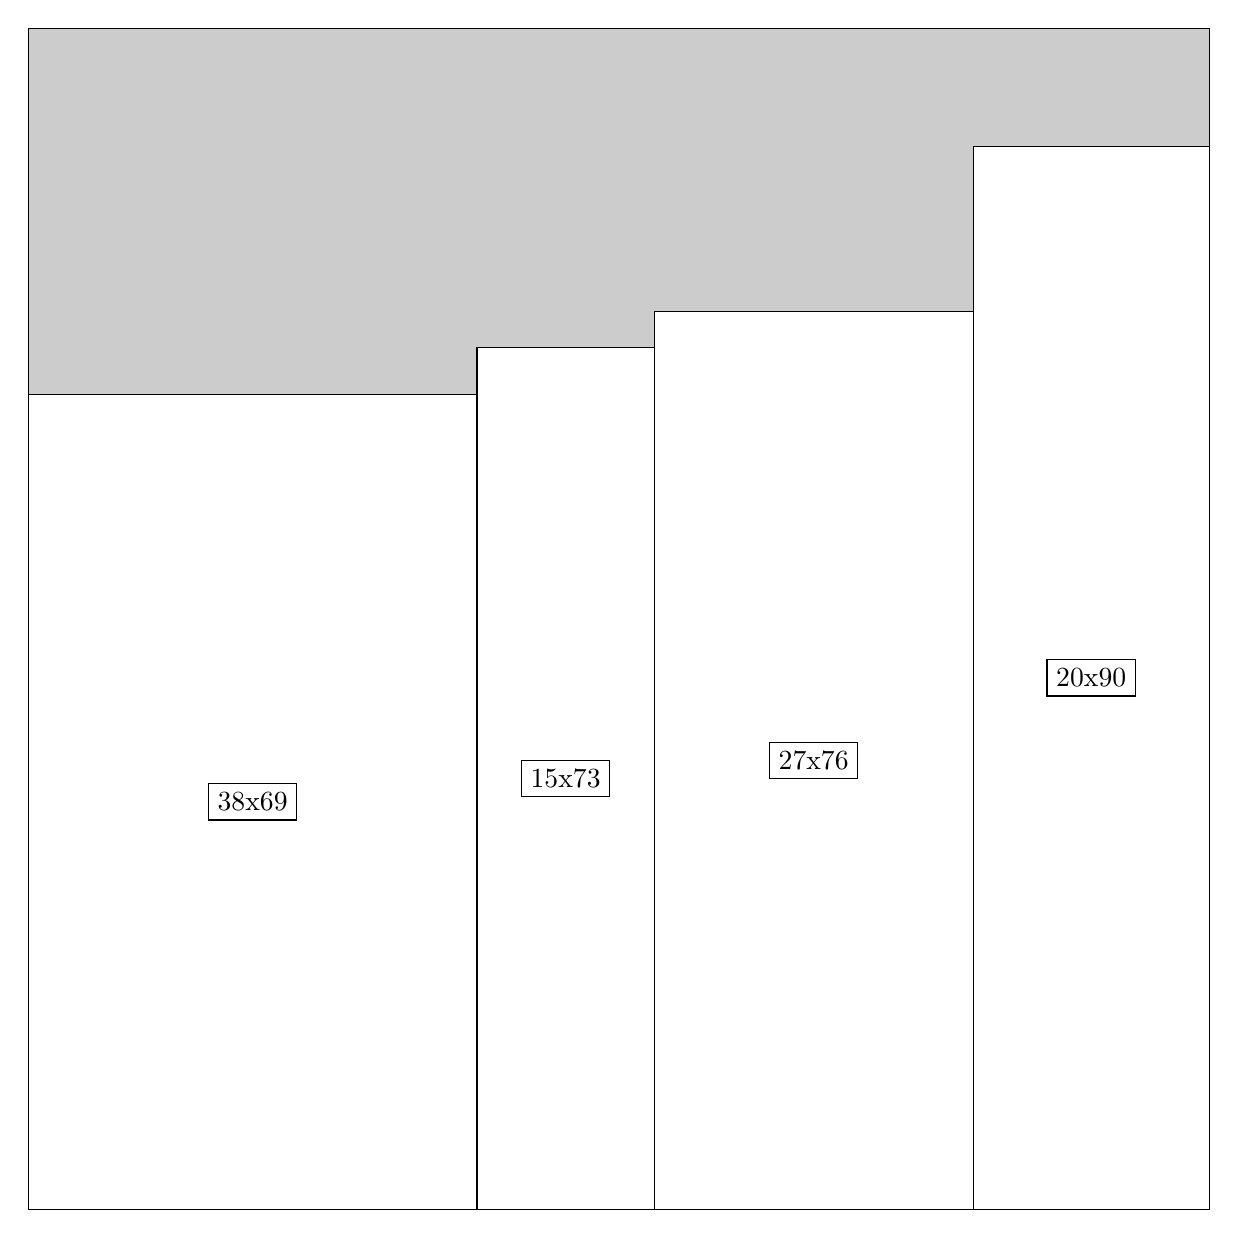
\begin{tikzpicture}[shorten >=1pt,scale=1.0,every node/.style={scale=1.0},->]
\tikzstyle{vertex}=[circle,fill=black!25,minimum size=14pt,inner sep=0pt]
\filldraw[fill=gray!40!white, draw=black] (0,0) rectangle (15.0,15.0);
\foreach \name/\x/\y/\w/\h in {20x90/12.0/0.0/3.0/13.5,27x76/7.949999999999999/0.0/4.05/11.4,15x73/5.7/0.0/2.25/10.95,38x69/0.0/0.0/5.7/10.35}
\filldraw[fill=white!40!white, draw=black] (\x,\y) rectangle node[draw] (\name) {\name} ++(\w,\h);
\end{tikzpicture}


w =20 , h =90 , x =80 , y =0 , v =1800
\par
w =27 , h =76 , x =53 , y =0 , v =2052
\par
w =15 , h =73 , x =38 , y =0 , v =1095
\par
w =38 , h =69 , x =0 , y =0 , v =2622
\par
\newpage


\end{document}